% !TEX program = pdflatex
% !TEX encoding = UTF-8 Unicode
% !TEX spellcheck = de-DE

% use KOMA class for cool presets like A4
\documentclass{scrartcl}

% load default packages for german and unicode support
\usepackage[ngerman]{babel}
\usepackage[T1]{fontenc}
\usepackage[utf8]{inputenc}

% load font to use (default linux libertine because it is a neat one
\usepackage{libertine}
\usepackage{libertinust1math}
\usepackage{subcaption}
\usepackage{graphicx}
\usepackage{blindtext}


% start with the actual content
\begin{document}
	\blindtext
	
% Füge die Bilder 3 mal hinzu, um sie dann per [h][t][b] unterschiedlich zu positionieren

	\begin{figure}[t]
	\begin{subfigure}{.3\textwidth}
		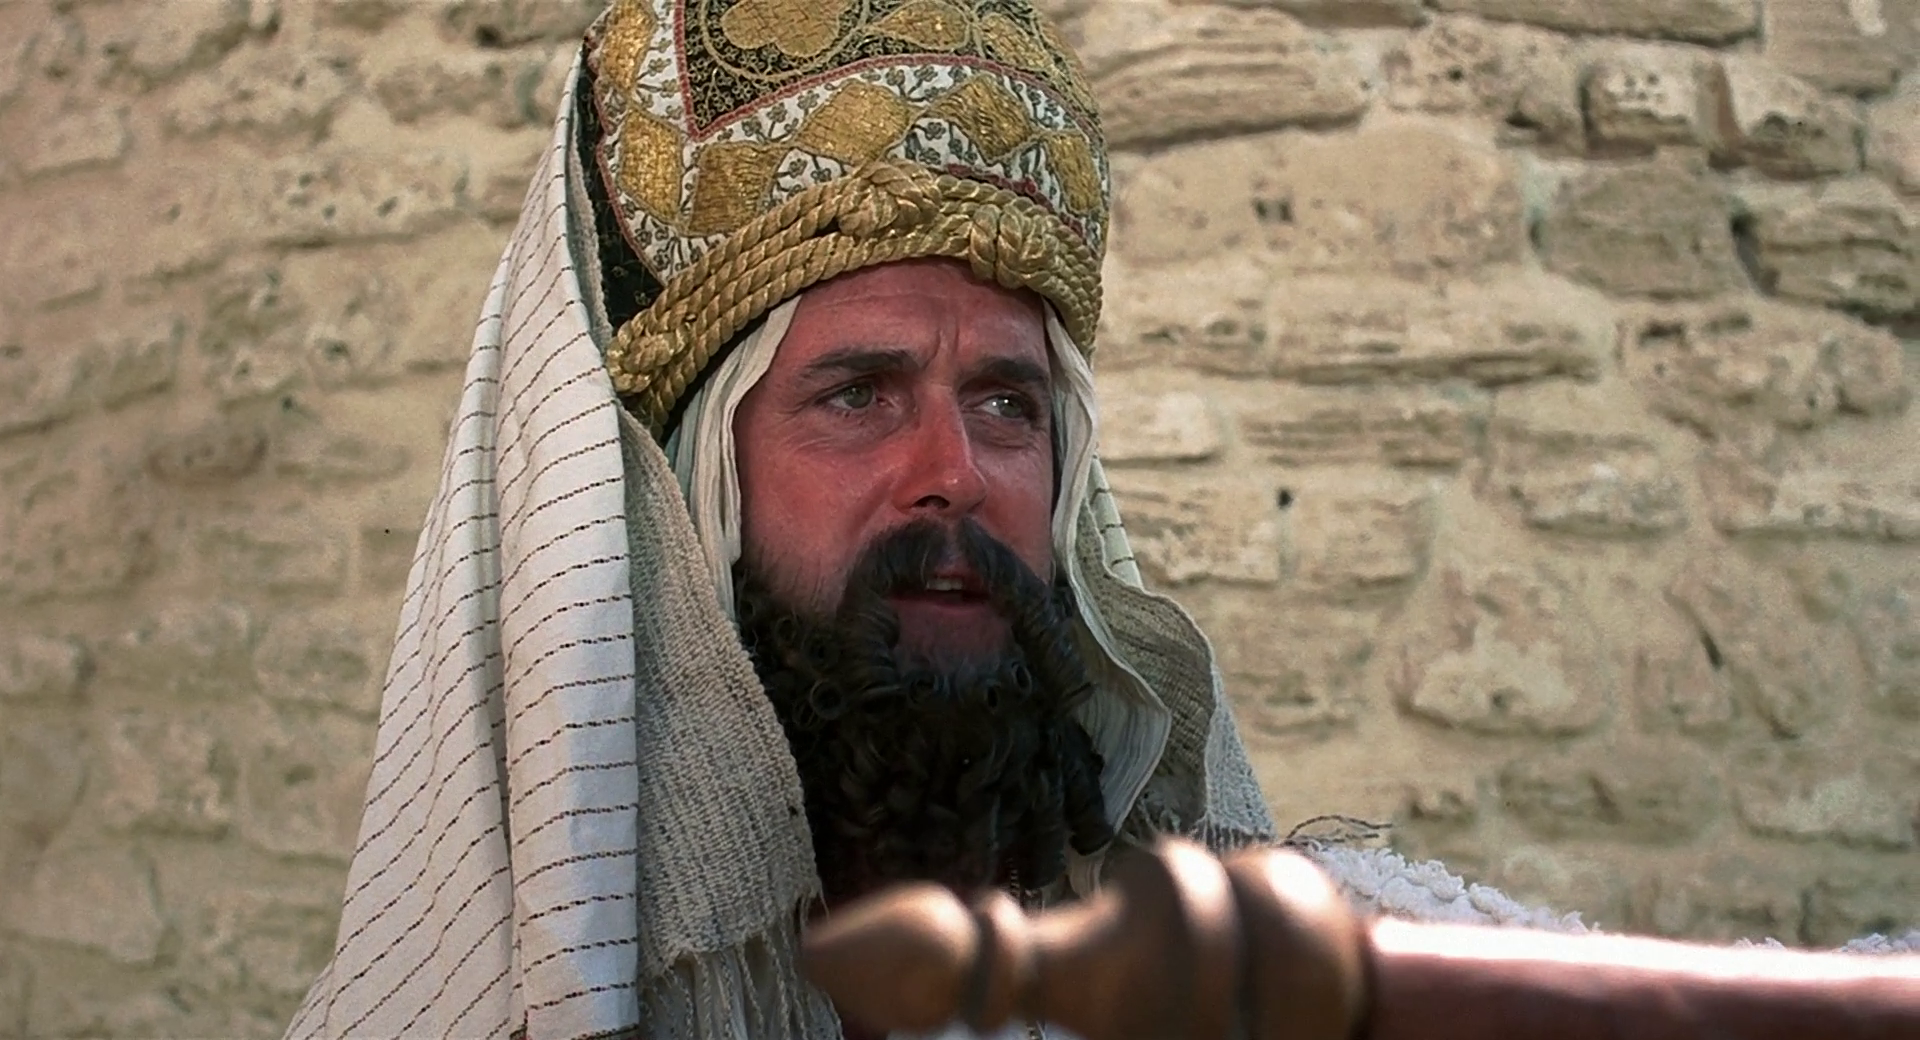
\includegraphics[width=\textwidth]{brian1}
		\caption{Hohepriester}
	\end{subfigure}
	\begin{subfigure}{.3\textwidth}
		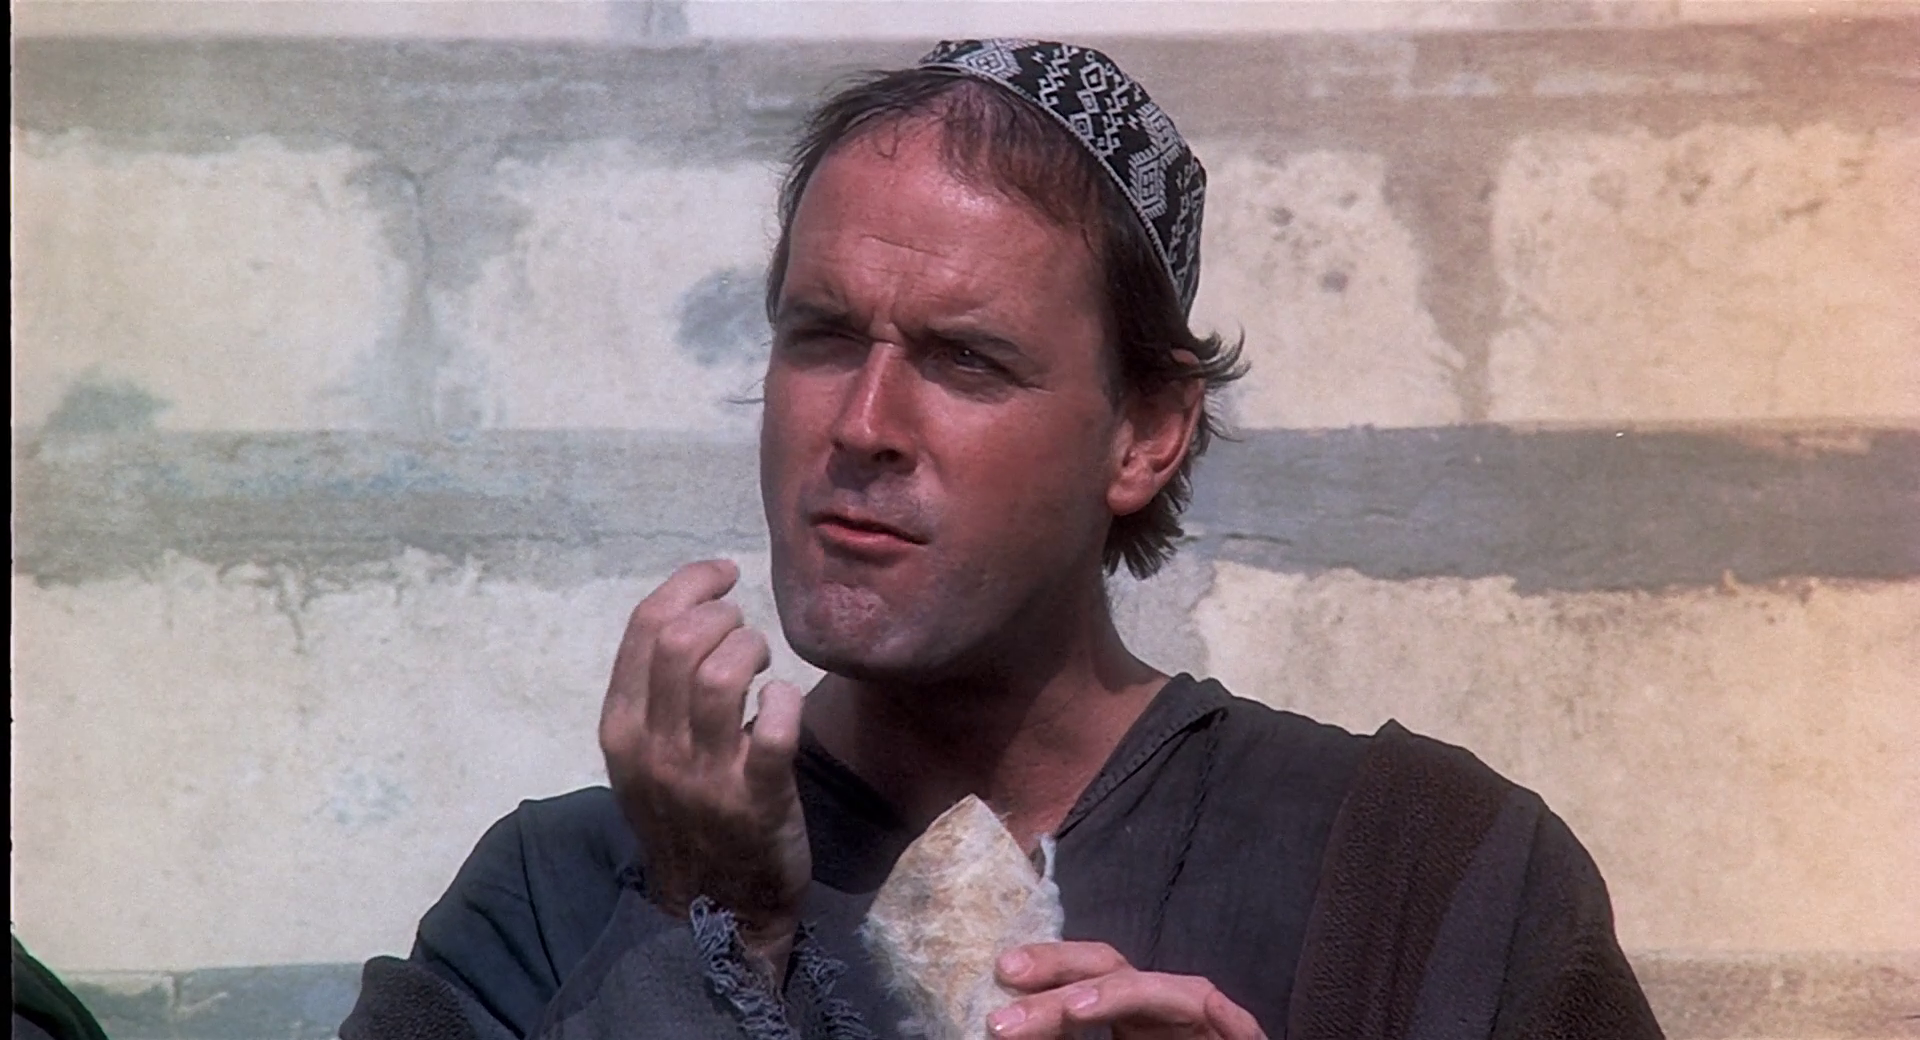
\includegraphics[width=\textwidth]{brian2}
		\caption{Reg}
	\end{subfigure}
	\begin{subfigure}{.333\textwidth}
		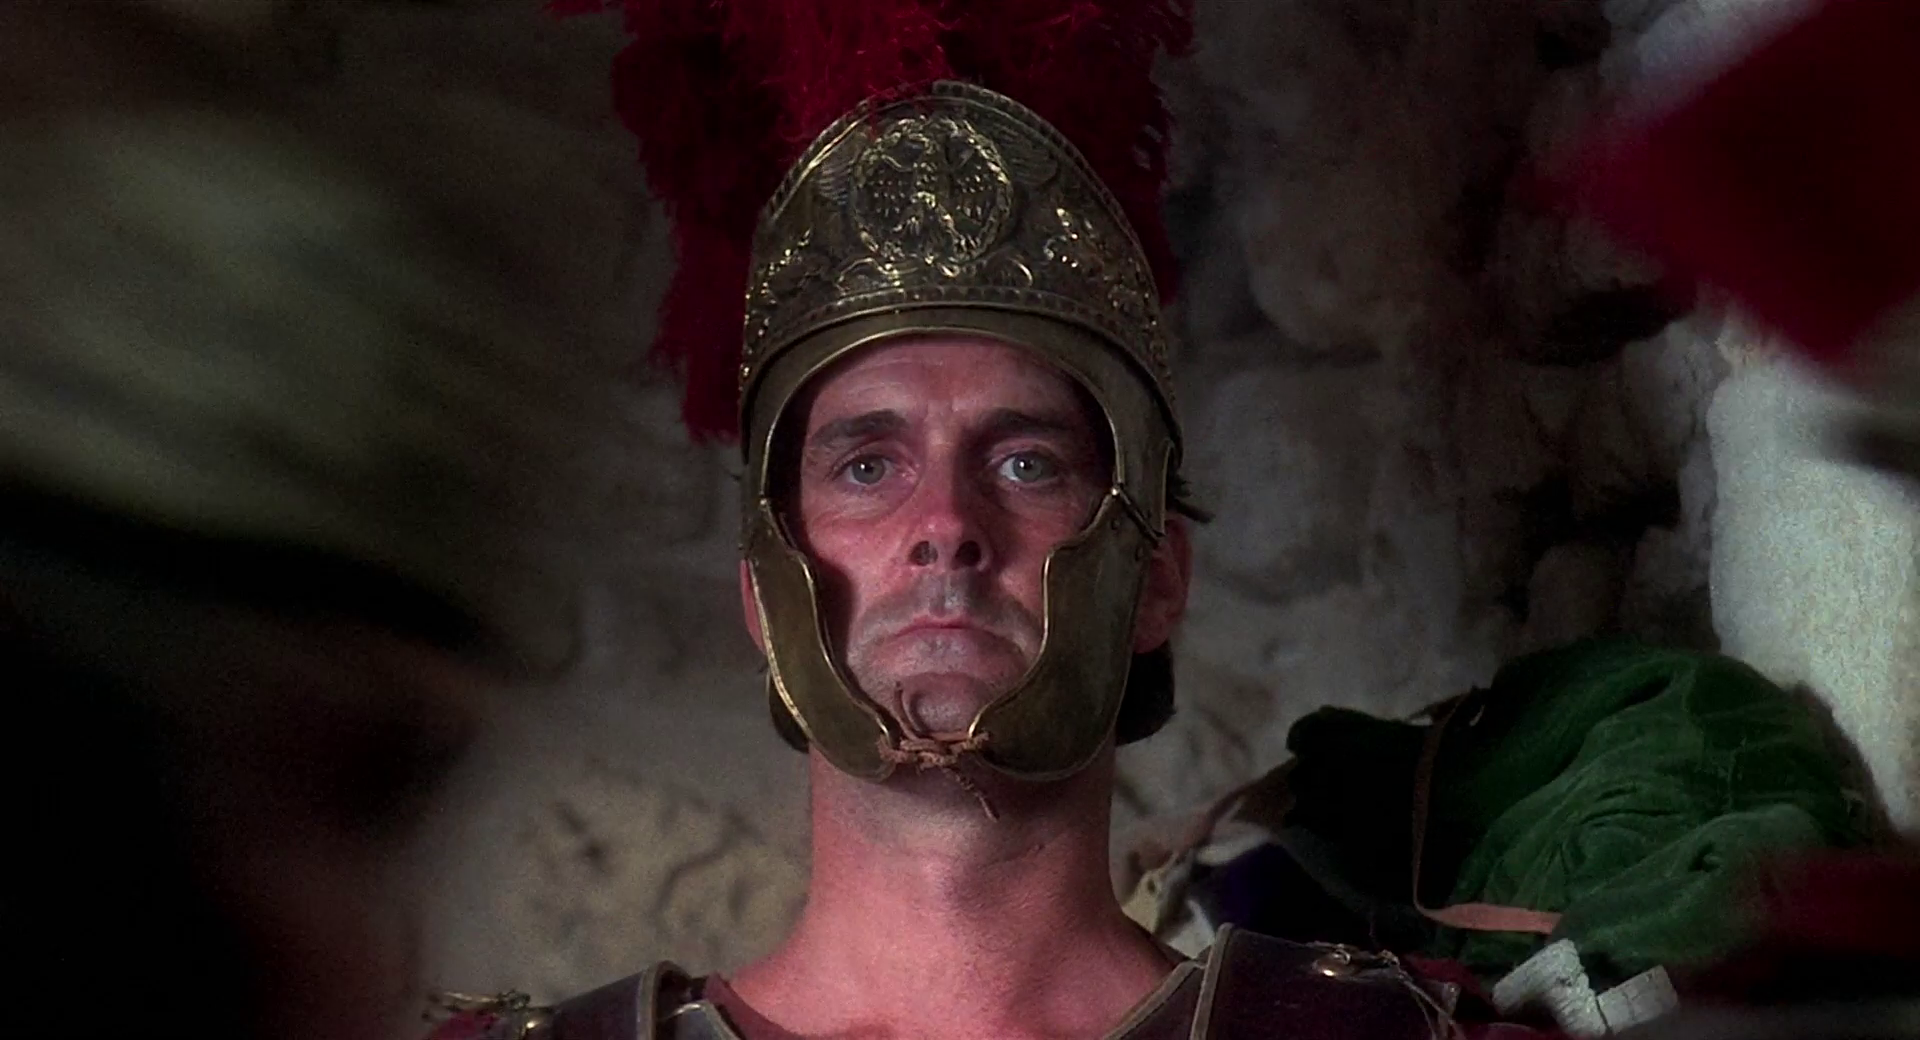
\includegraphics[width=\textwidth, height=24mm]{brian3}
		\caption{Centurio}
	\end{subfigure}
	\caption{John Cleese porträtiert den minimalen, antiken Genpool}		
    \end{figure}


	\begin{figure}[h]
	\begin{subfigure}{.3\textwidth}
		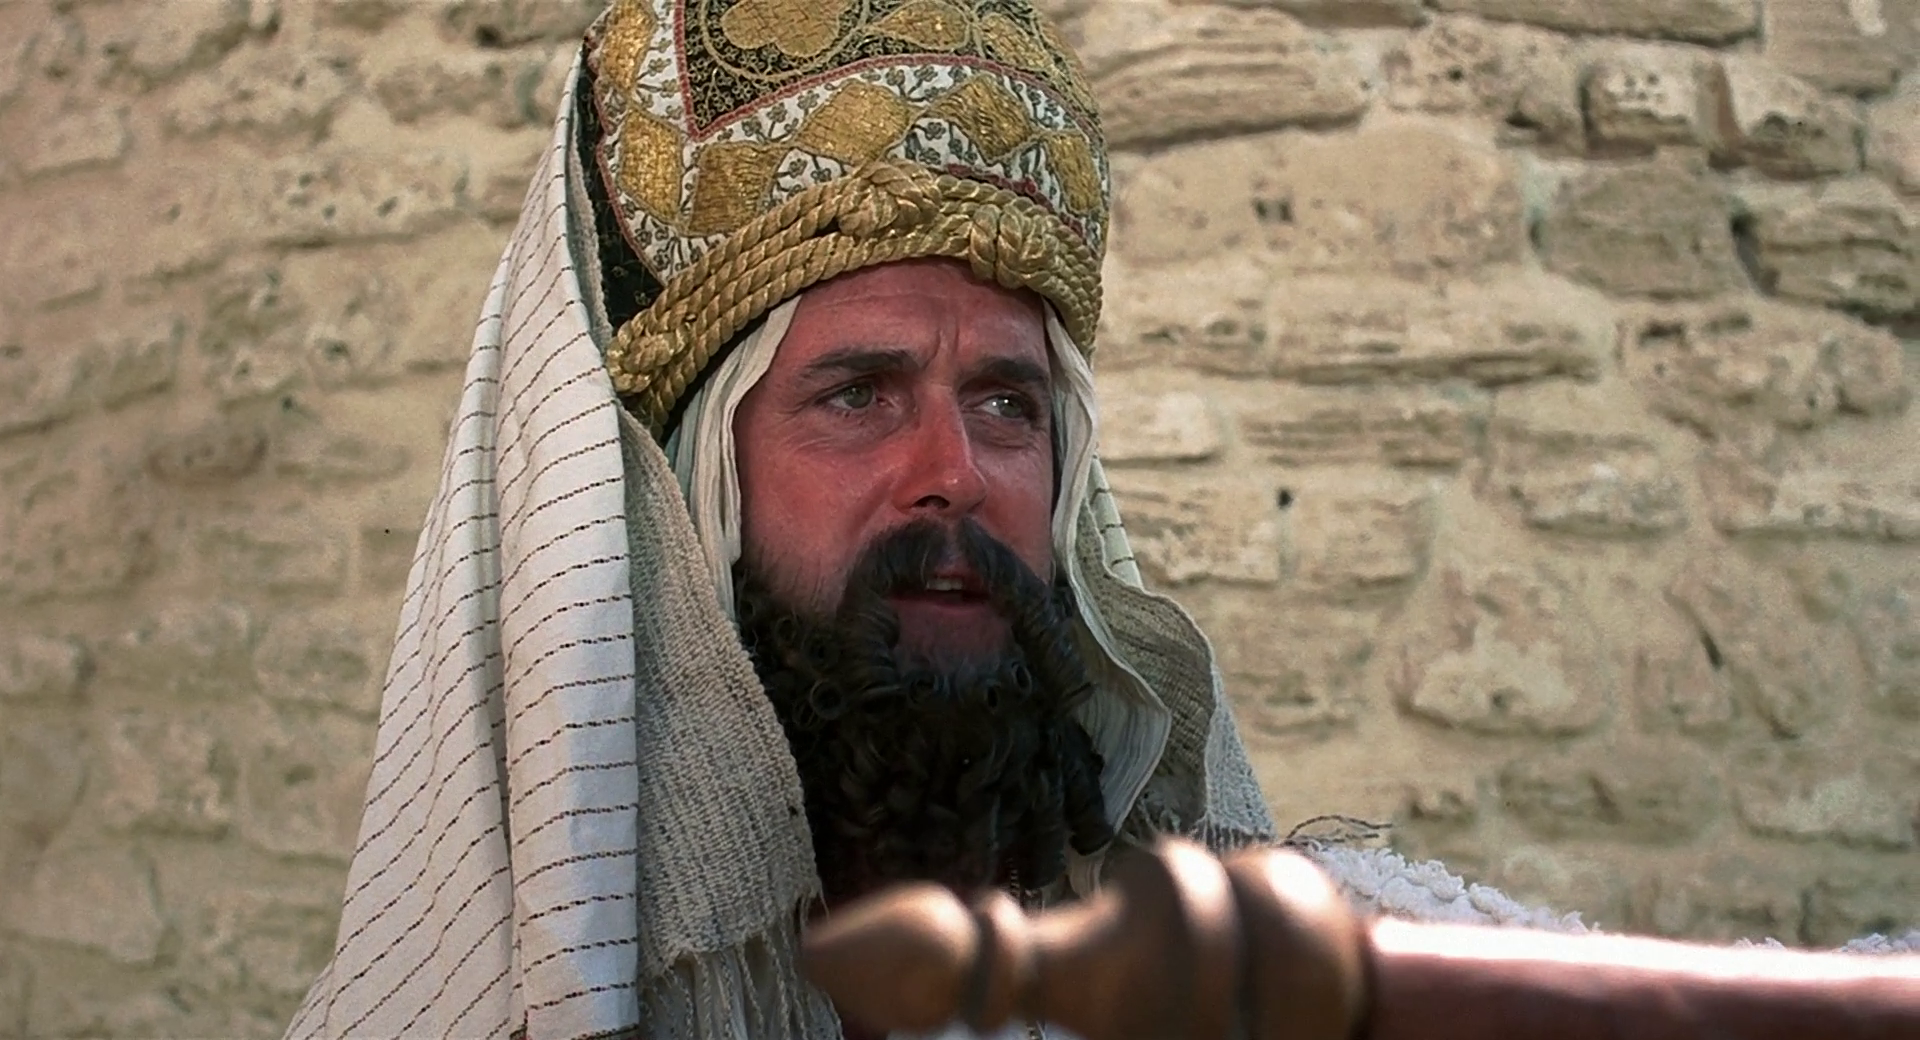
\includegraphics[width=\textwidth]{brian1}
		\caption{Hohepriester}
	\end{subfigure}
	\begin{subfigure}{.3\textwidth}
		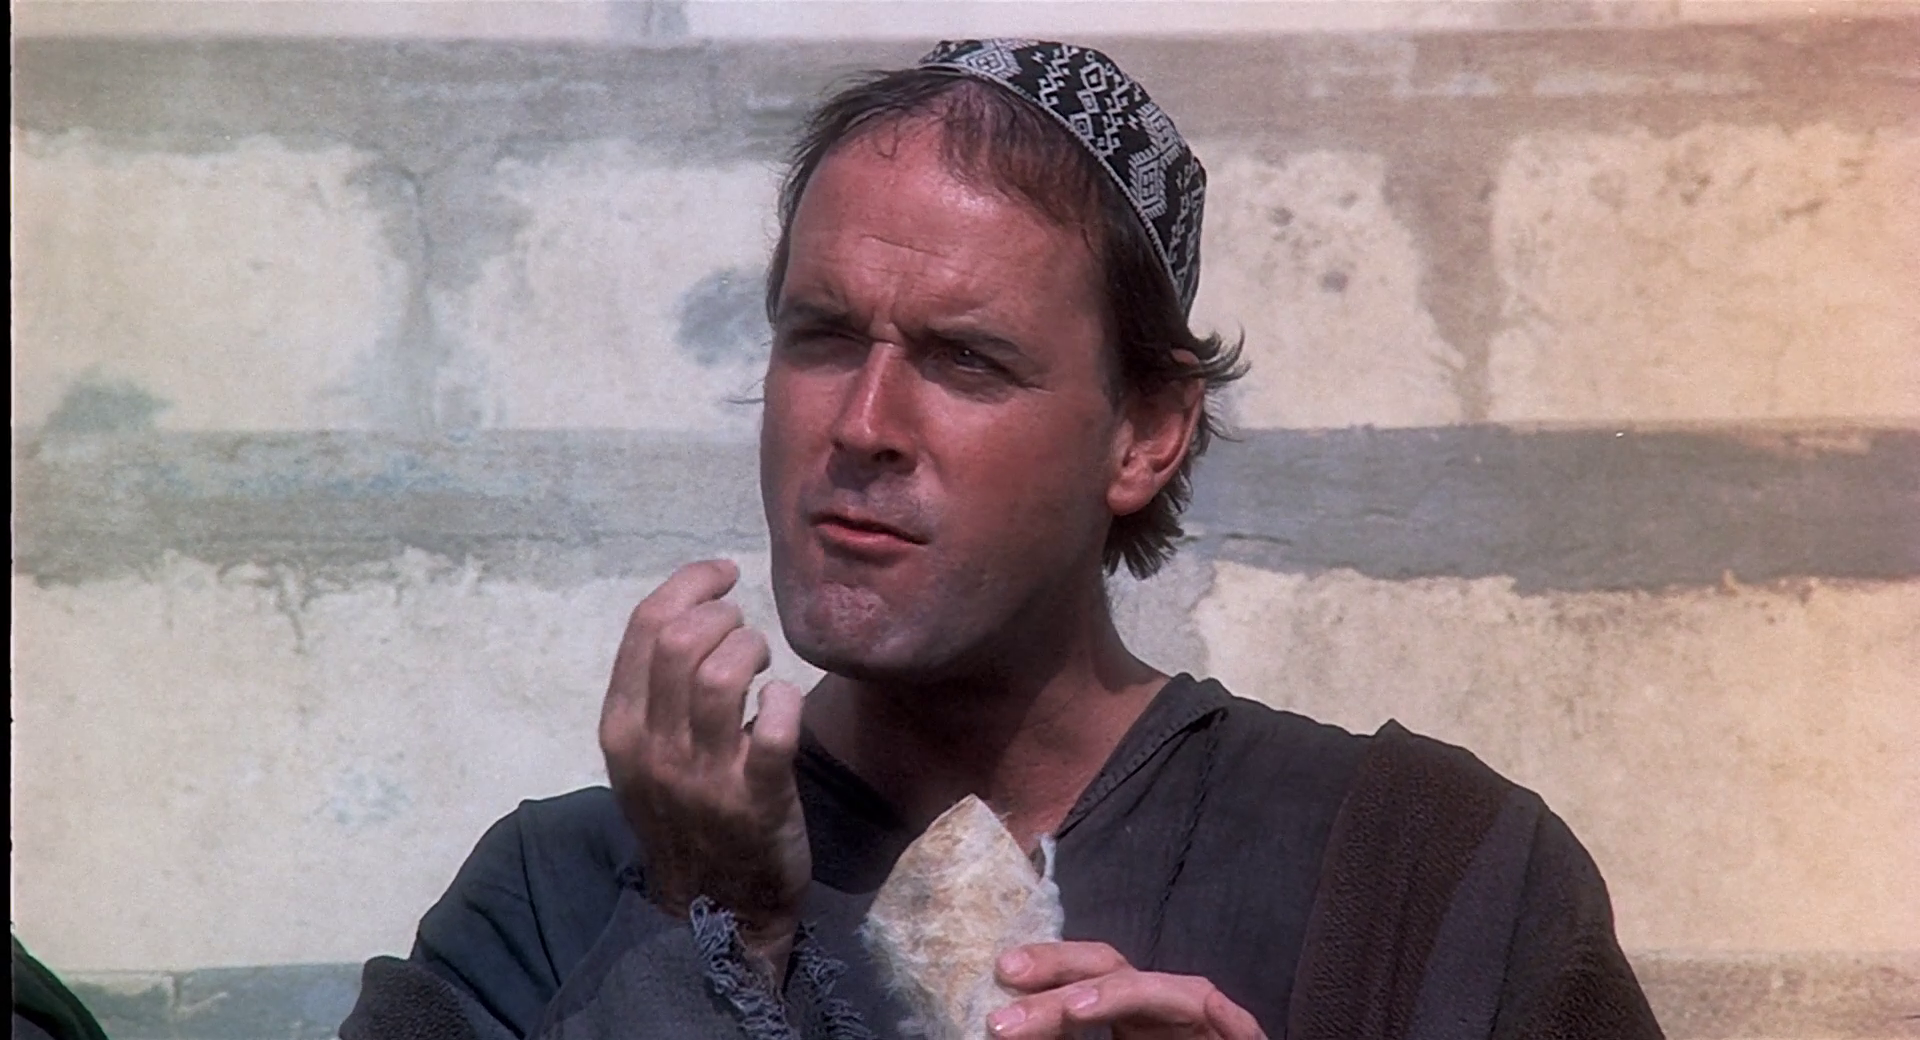
\includegraphics[width=\textwidth]{brian2}
		\caption{Reg}
	\end{subfigure}
	\begin{subfigure}{.333\textwidth}
		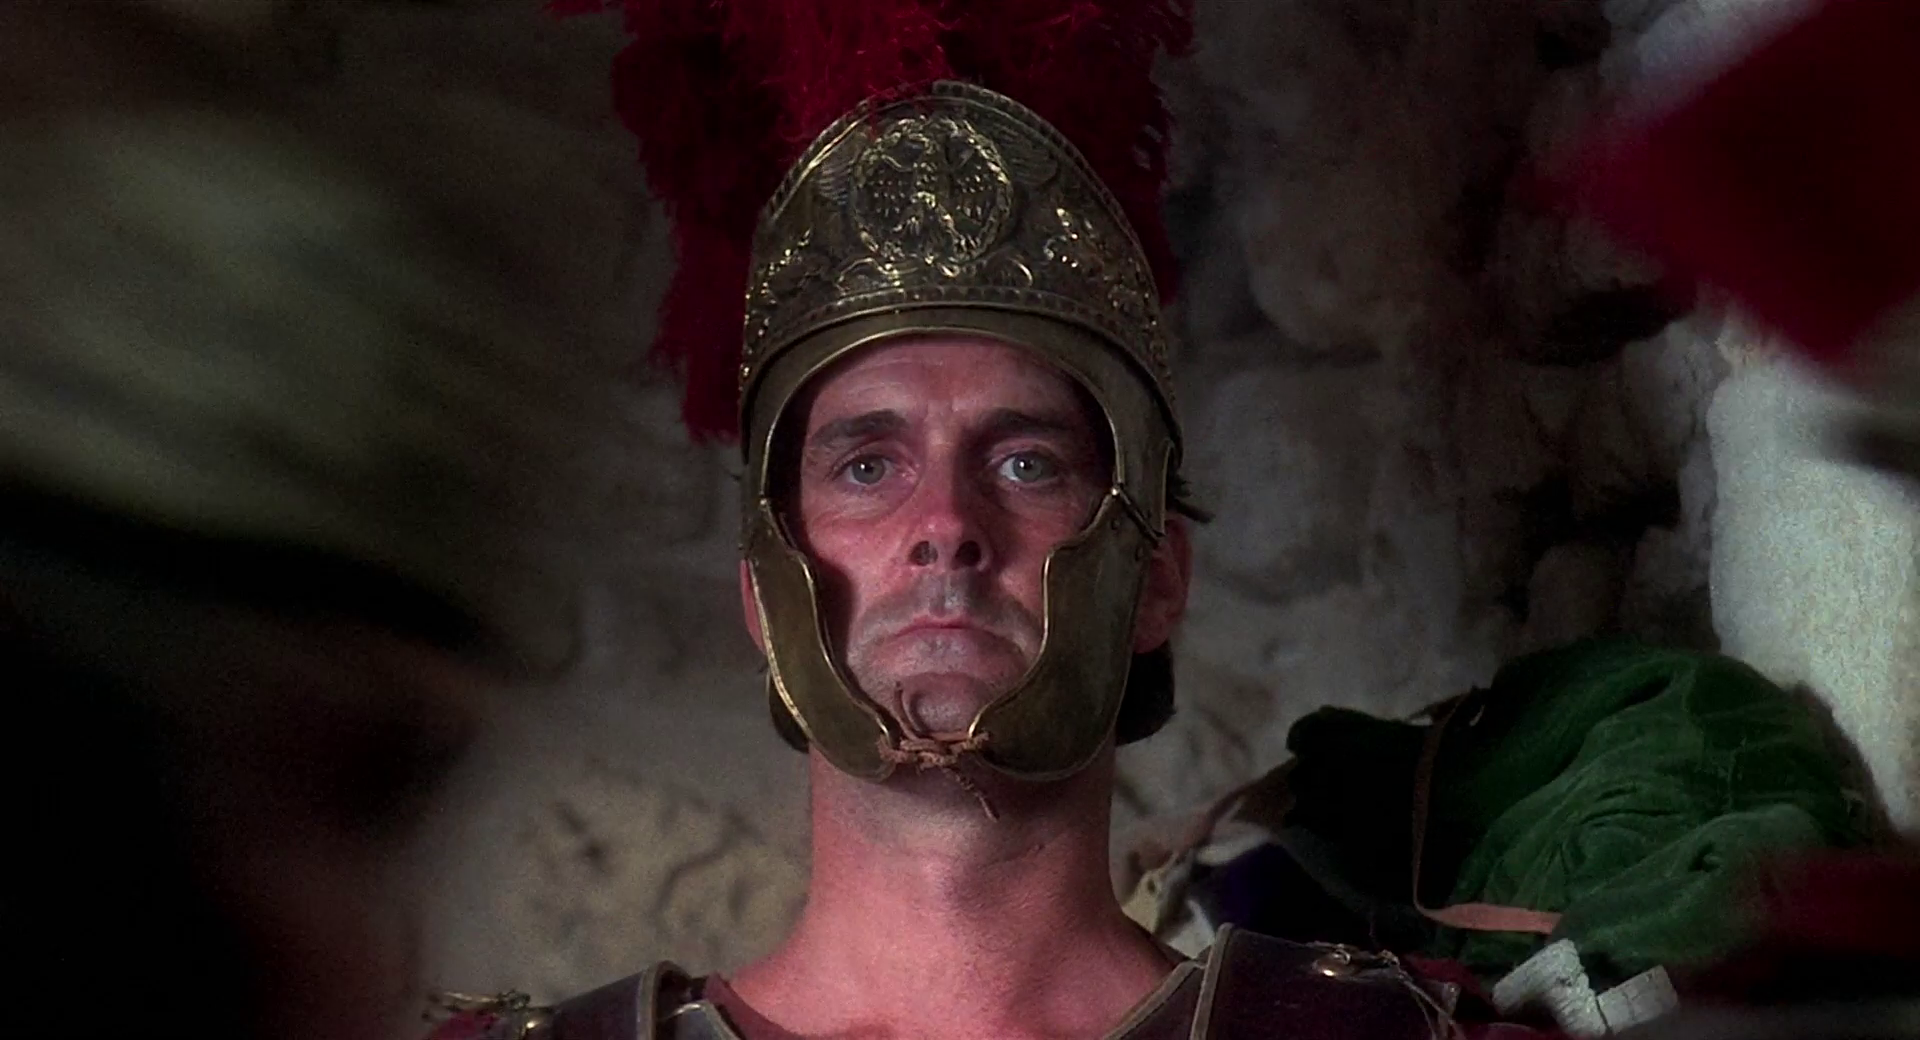
\includegraphics[width=\textwidth, height=24mm]{brian3}
		\caption{Centurio}
	\end{subfigure}
	\caption{John Cleese personifiziert den minimalen, antiken Genpool}		
    \end{figure}



	\begin{figure}[b]
		\begin{subfigure}{.3\textwidth}
				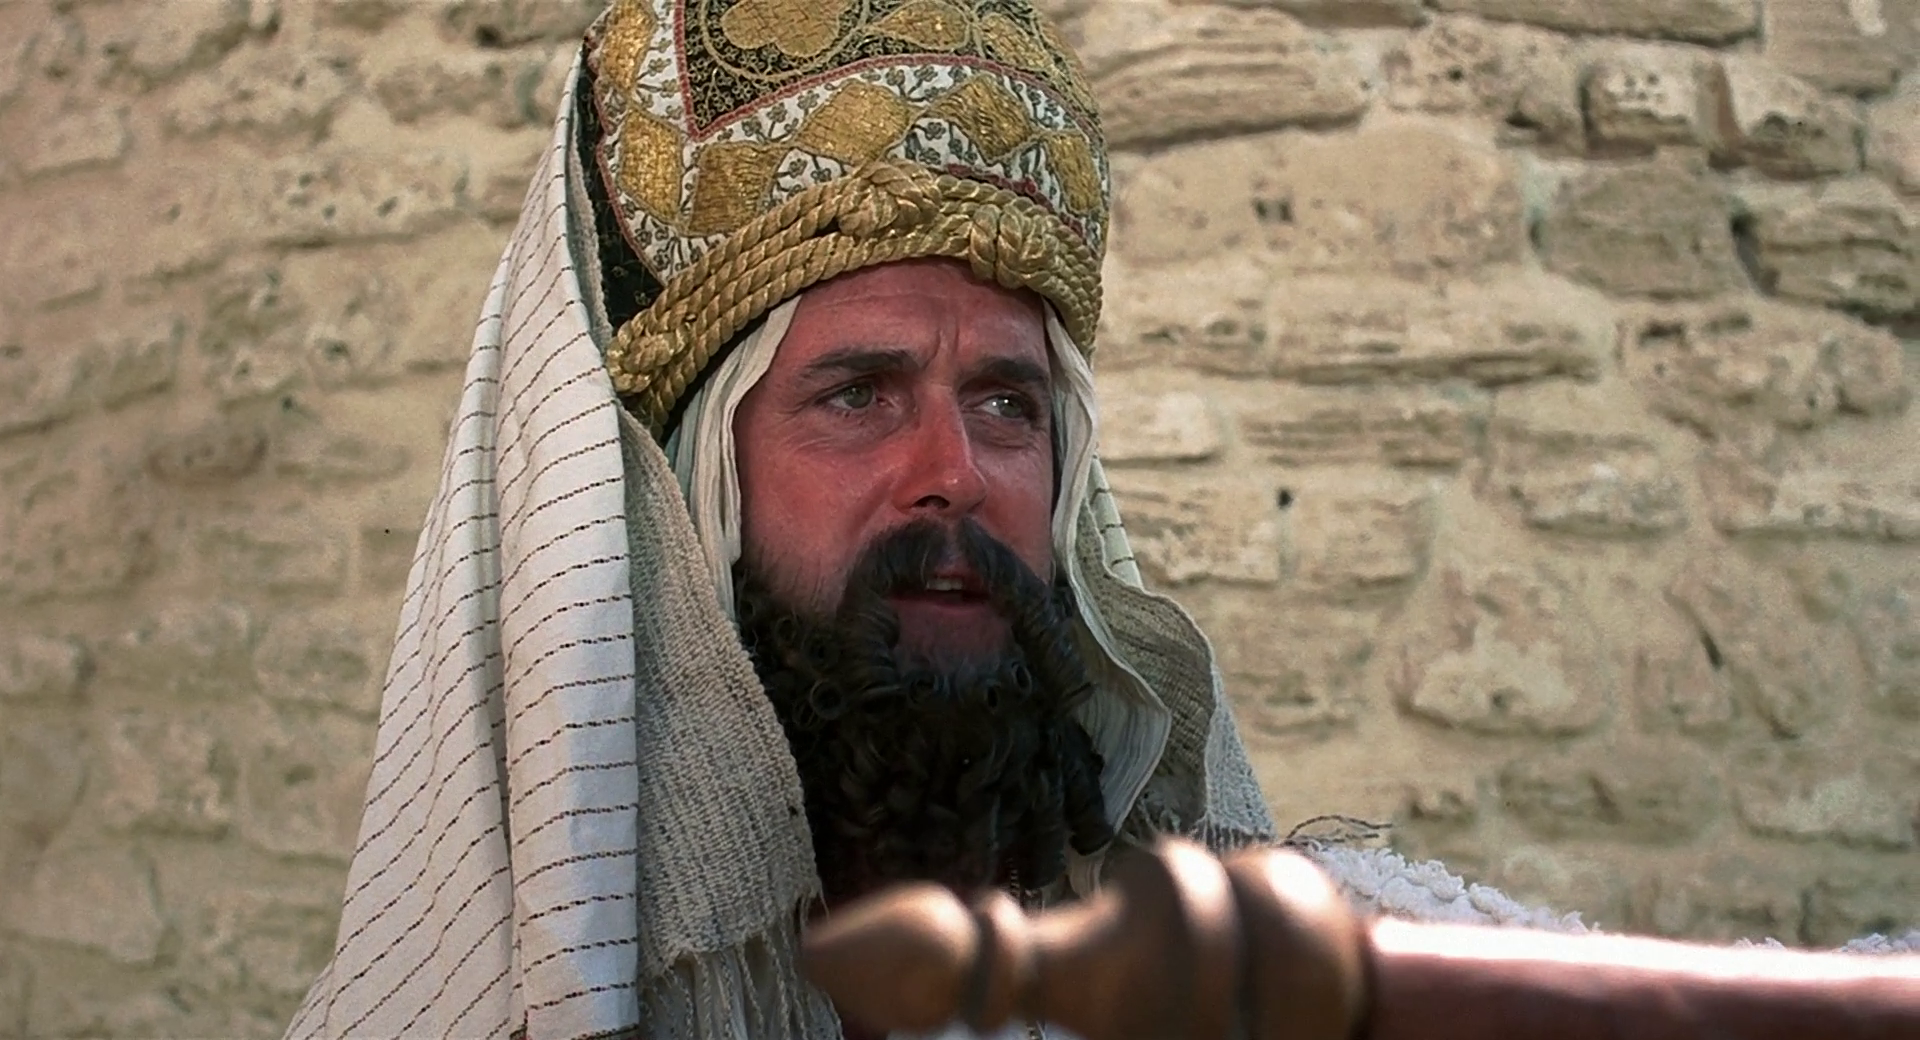
\includegraphics[width=\textwidth]{brian1}
			    \caption{Hohepriester}
		\end{subfigure}
	    \begin{subfigure}{.3\textwidth}
	    	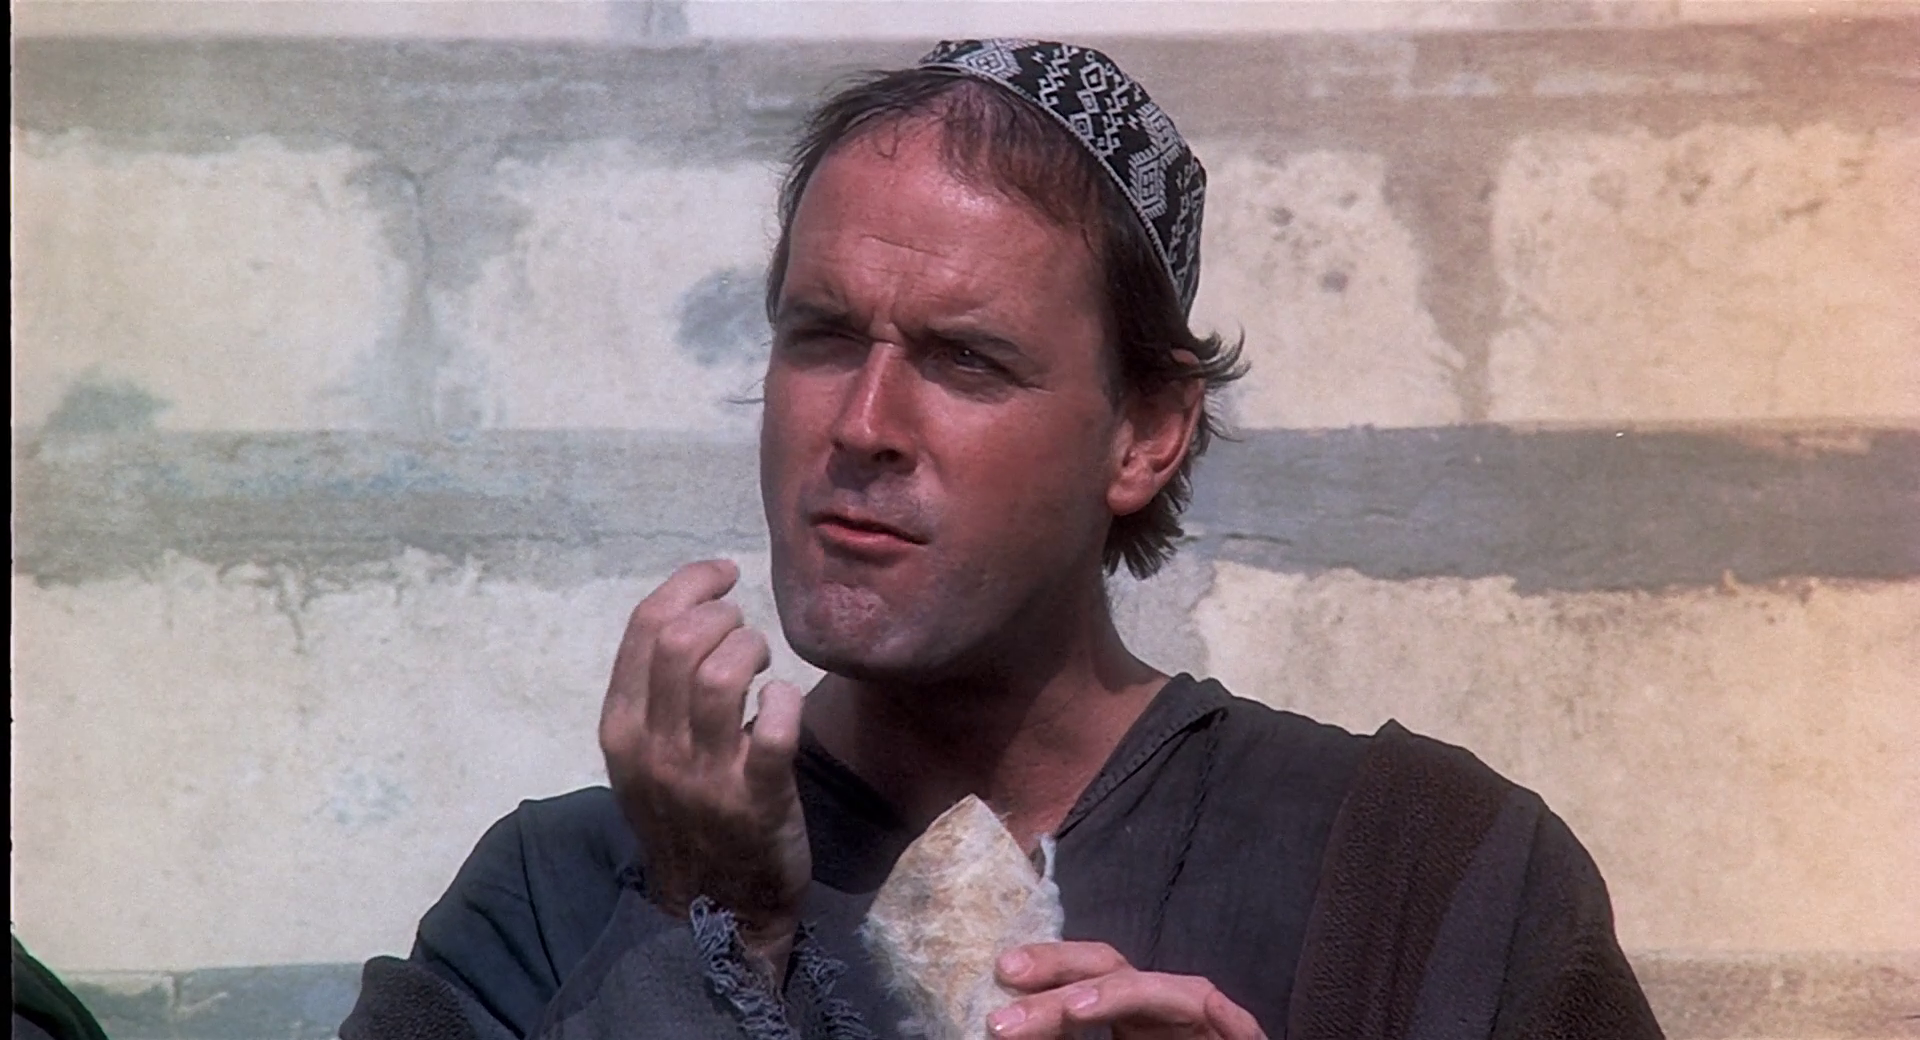
\includegraphics[width=\textwidth]{brian2}
	    	\caption{Reg}
	    \end{subfigure}
        \begin{subfigure}{.333\textwidth}
        	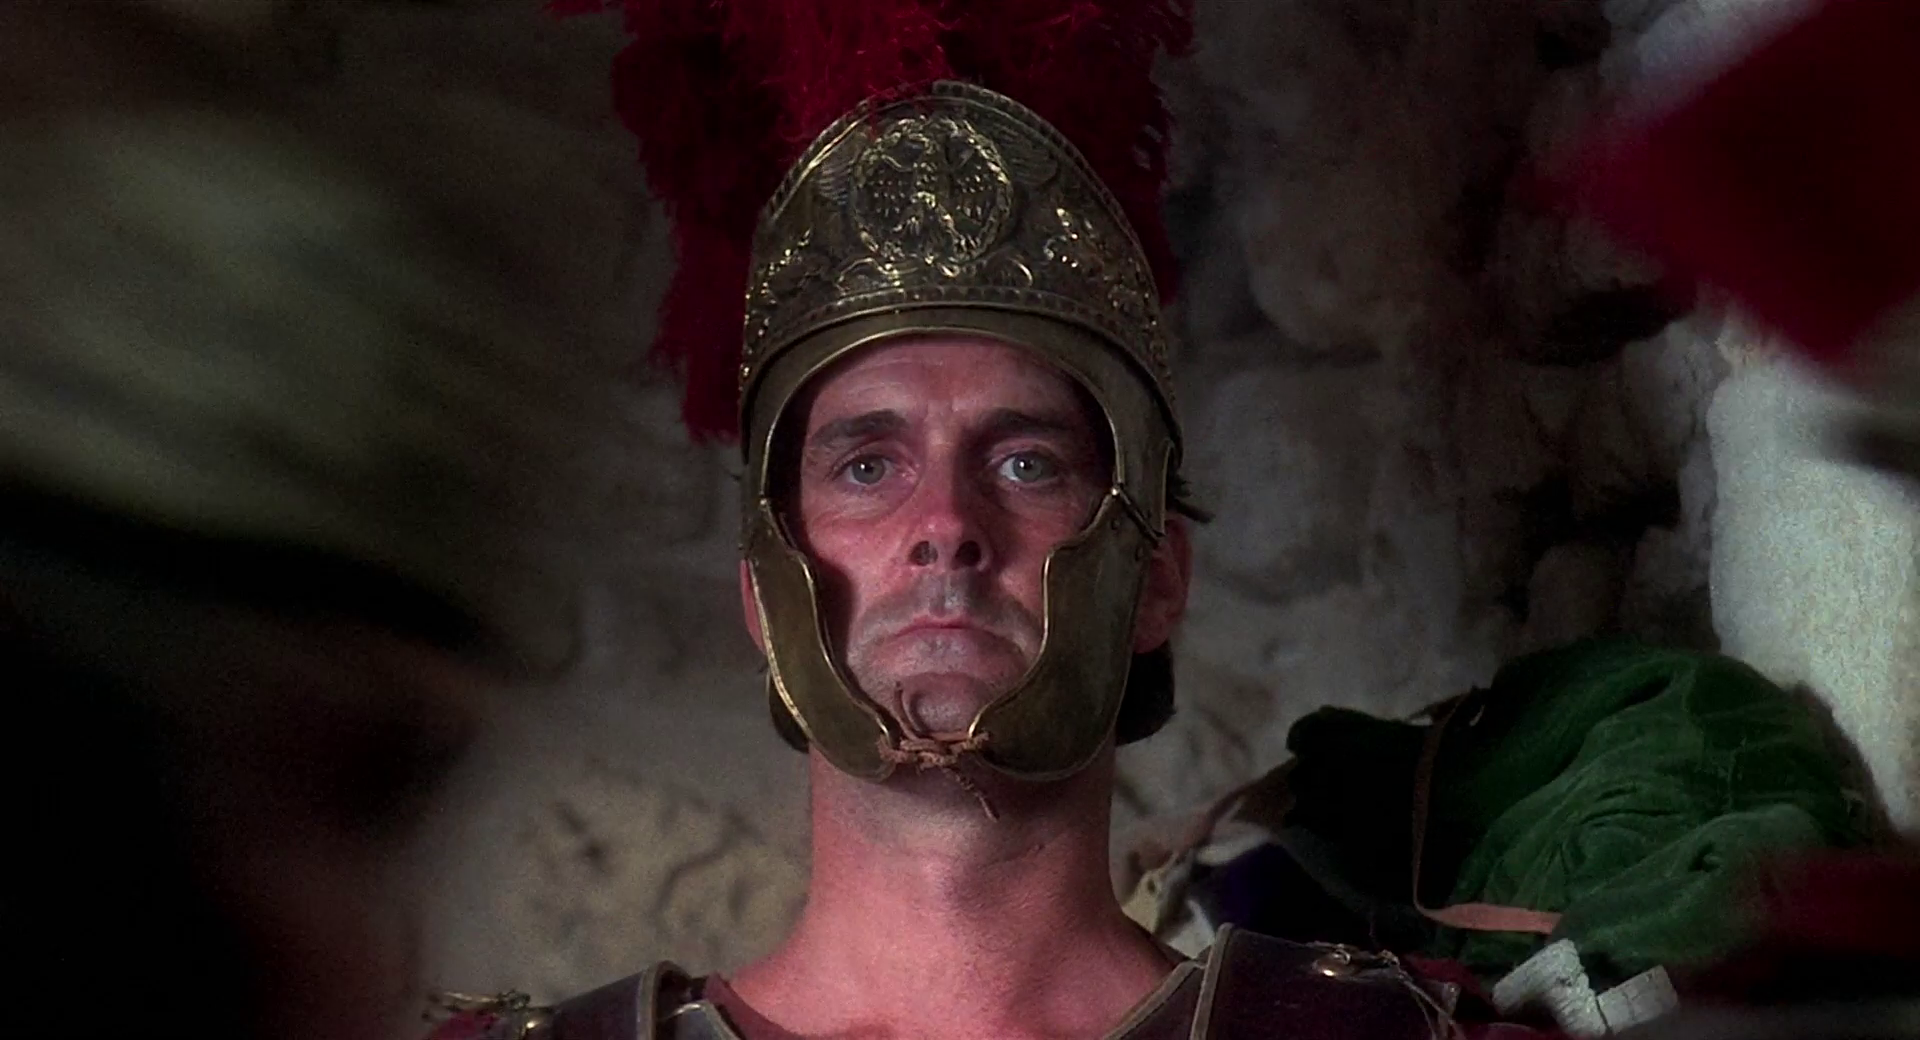
\includegraphics[width=\textwidth, height=24mm]{brian3}
        	\caption{Centurio}
        \end{subfigure}
    \caption{John Cleese stammt aus dem minimalen, antiken Genpool}		
	\end{figure}


\blindtext


\begin{figure}[h]
	\centering
	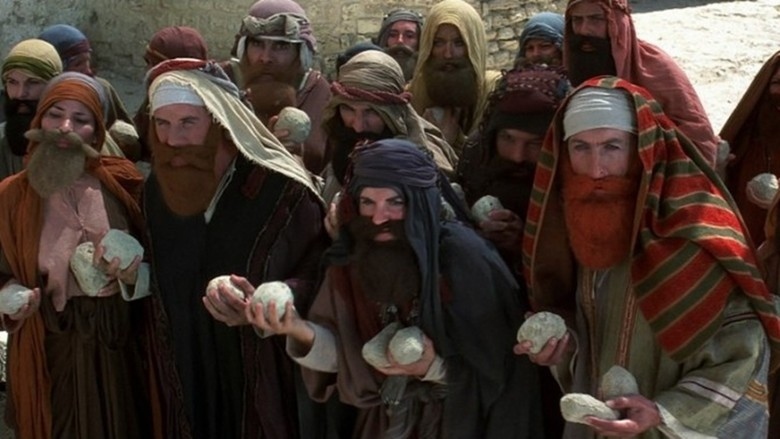
\includegraphics[angle=5, width=7cm]{brian4}
	\caption{Ein Beispiel eines rotierten Bildes}
\end{figure} 

Allerdings sieht das rotierte Bild reichlich unpassend aus.
% end of written content
\end{document}

% vim: ft=tex et sw=2 tw=80:
